\subsection{Electric Circuits} 

%\DTMnewdatestyle{dateupdated}{〈definition 〉

Answers to M\Alph{subsection} problems are on page \pageref{circuit_prob_answers}.  \textbf{\textcolor{red}{Updated \DTMnow.}}

%--------------------------------------------------------------------------------------------------------------
\begin{Exercise}
\label{road_construction_problem}
Road construction to fix a break in an underground sewer line has caused a long backup on a state highway.  There's a single line of cars backed up for six miles, traveling at an average speed of just four miles per hour.  There are 250 cars per mile along the road.  
(a)~How many cars pass the construction site every hour?  
(b)~Write a general expression for the number of cars that pass a given spot on the road per time in terms of the number of cars per length of road and the average speed $v_\text{avg}$ of the cars.
\end{Exercise}
\begin{Answer}
(a)~1000 cars per hour 
(b)~(\# cars per time) = (cars per length) $\times~v_\text{avg}$.\end{Answer}


%--------------------------------------------------------------------------------------------------------------
\begin{Exercise}
The density of water is 1~g/cm$^3$, which works out to a ``number density'' of $n_\text{w}=3.34 \times 10^{28}$ molecules per cubic meter.  Suppose a water pipe has a cross-sectional area of $A=5 \text{~cm}^2$.  
(a)~How many water molecules are there in a section of pipe of length $L=2.5$~ meters?  
(b)~How many water molecules are there per meter of length in the pipe?  
(c)~Write a general expression for the number of water molecules per length of pipe in terms of $n_\text{w}$ and $A$.  
(d)~If the speed of water flowing in the pipe is $v_\text{avg}=1.8$~m/sec, how many molecules pass through a given spot in the pipe every second?  Hint: your result from problem \ref{road_construction_problem} is applicable here.  
(e)~Write a general expression for the number of water molecules flowing per time in terms of $n_\text{w}$, $A$, and $v_\text{avg}$.
\end{Exercise}
\begin{Answer}
(a)~$4.18  \times 10^{25}$ molecules 
(b)~$1.67 \times 10^{25}$ molecules per meter 
(c)~(\# molecules per length) $= n_\text{w} A$  
(d)~$3.0 \times 10^{25}$ molecules per second  
(e)~\# molecules per time $= n_\text{w} Av_\text{avg}$
\end{Answer}


%--------------------------------------------------------------------------------------------------------------
\begin{Exercise}
In the first circuit lab you did (Lab \ref{lab_circuits1}), a typical current through one light bulb was about 70~mA.  
(a)~If you kept the bulb on continuously, how many electrons would enter the bulb every hour? 
(b)~How many electrons would leave the bulb every hour?  
(c)~For the sake of comparison, how many electrons are contained in the actual light bulb filament, a small tungsten wire with a mass of about 2~mg? 
(Hint: a typical tungsten atom off the street has 110~neutrons and 74~protons).
\end{Exercise}
\begin{Answer}
My number for (a) and (b) is 3.3 times my number for (c)
\end{Answer}


%--------------------------------------------------------------------------------------------------------------
\begin{Exercise}
The wires in your home are probably made of copper (resistivity $\rho = 1.7 \times 10^{-8} \Omega \cdot \text{m}$) and would have a cross-sectional area of 3.3~mm$^2$ assuming it's the common ``12-gauge'' stuff.%
\footnote{The American Wire Gauge system, or ``AWG,'' is among the more idiosyncratic  systems of units you will see---starting with its pronunciation, where ``gauge'' rhymes with \textit{page}.  Increasing wire diameter is denoted by \textit{decreasing} gauge number, from ``40~gauge'' (0.00314-inch diameter) to ``0~gauge'' (0.3249-inch diameter)---except that there are additional thicker gauges denoted by multiple zeros, down to ``0000 gauge'' for 0.4600-inch-diameter wire.  The system is logarithmically stepped, meaning that the ratio of the diameters of any two successive gauge numbers is the same---a ratio that is defined to be $\sqrt[39]{92}$, because of course it is. Historically, the American Wire Gauge system is based on a nearly identical gauge system used for sheet metal in the late 1800s by the Brown \& Sharpe machine tool company, located on a 33-acre parcel of land on the Woonasquatucket River in Rhode Island.}
(a)~What is the conductivity $\sigma$ of copper? 
(b)~If the electric field inside one of the wires is $6 \times 10^{-3}~$V/m, find the current $I$ through the wire. 
(c)~Assuming there is one free electron per copper atom, the density of free electrons works out to be $n_e = 8.5 \times 10^{28} \text{m}^{-3}$.  If that's true, what is the drift velocity of the electrons for the current you found in (b)? 
(d)~Estimate the mean time between collisions in copper.  
\end{Exercise}
\begin{Answer}
(a)~$5.9 \times 10^7 ~\Omega^{-1}\text{m}^{-1} $
(b)~1.16 amps 
(c)~$2.6 \times 10^{-5}$ m/s 
(d)~$2.46 \times 10^{-14}$ s
\end{Answer}


%--------------------------------------------------------------------------------------------------------------
\figuretoright{0.40}{M_problems/circuits/four_resistor_circuit.pdf}{
\begin{Exercise}
Find the current in each resistor in the circuit to the right.  
\end{Exercise}
\begin{Answer}
$I_{2\Omega}=I_{4\Omega}=2.67~\text{A};
 I_{3\Omega}=0.67~\text{A}; 
 I_{1\Omega}=2.0~\text{A}$
\end{Answer}


%--------------------------------------------------------------------------------------------------------------
\begin{Exercise}
For the circuit shown to the right (same picture as the previous problem), find (a)~the power delivered to each resistor, and (b)~the total power delivered by the battery. 
\end{Exercise}
\begin{Answer}
(a) $P_{2\Omega}=14.22$~W; $P_{4\Omega}=28.44$~W; $P_{3\Omega}=1.33$~W; $P_{1\Omega}=4$~W  (b)~48 W
\end{Answer}
}

%--------------------------------------------------------------------------------------------------------------
\begin{Exercise}
A pair of students is measuring the current and voltage across a tiny, nominally $100\ohm$ resistor. They obtain the following data:

\begin{center}
\begin{tabular}{|C{1in}|C{1in}|C{1in}|C{1in}|C{1in}|}
\hline
Measured $V$	&Measured $I$ & Calculated $P$	& Calculated $R$	& How hot? \\
\hhline{|=|=|=|=|=|}
1.253 volts&	0.01261 amps&	15.8 mW&	$99.37\ohm$ &	not hot\\ \hline
9.84 volts	&0.0962 amps	&947 mW& $102.29\ohm$ &	HOT!\\ \hline
\end{tabular}
\end{center}
Anna says ``Hey, cool!  It looks like the resistance increased when it got hot. That means the resistor has a positive temperature coefficient.''  Bob says, ``Gee, I dunno.  That's a pretty small difference.  I don't really think that counts.'' After scratching their heads for a while, they look in the manual for their multimeters and find that their current and voltage measurements all have an uncertainty of 0.5\%.  
(a) Calculate the uncertainty in the resistances they measured.  
(b) Is the difference between their two calculated resistance values significant? 
Hint: see Appendix~\ref{uncertainty} for a refresher on analyzing uncertainties.
\end{Exercise}
\begin{Answer}
Partial answer: Properly combining the uncertainties for $V$ and $I$ in quadrature for the first resistor gives an uncertainty of about $\pm 0.7\ohm$.
\end{Answer}


%--------------------------------------------------------------------------------------------------------------
\begin{Exercise}
For the circuit shown below, (a)~What is the current in the $20\ohm$ resistor?  (b)~What is the potential difference between points a and b?  (Hint: you'll need to redraw this circuit to make it more obvious which resistors are in parallel or series with each other.  You may want to make several iterations of drawings.) 
\begin{center}
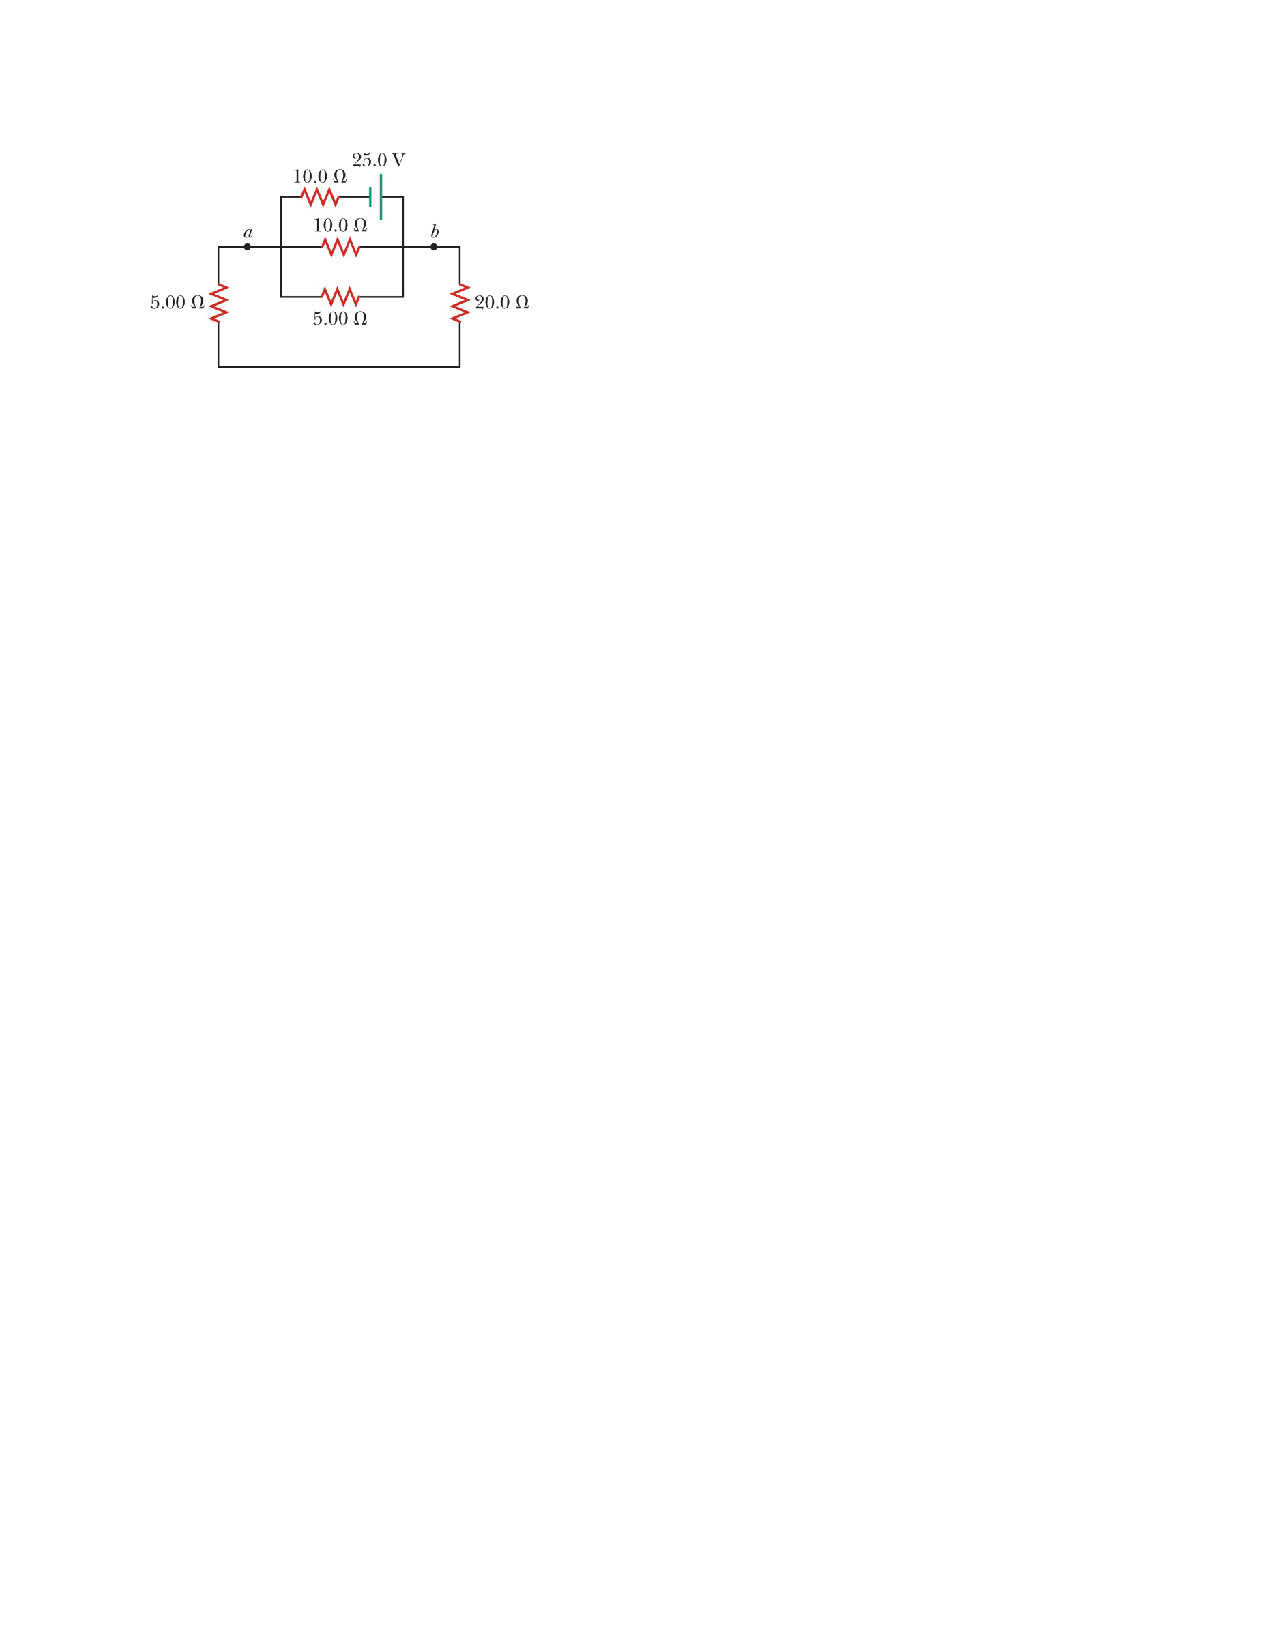
\includegraphics{M_problems/circuits/goofy_circuit.pdf}
\end{center}
\end{Exercise}
\begin{Answer}
(a) 227 mA (b) 5.68 V
\end{Answer}


%--------------------------------------------------------------------------------------------------------------
\begin{Exercise}
Three resistors, each with $R=100\ohm$, are connected as shown.  Each resistor has a maximum power rating of 25~watts.  
(a)~What is the maximum voltage that can be applied between the terminals a and b?  
(b)~At that voltage, what is the total power delivered to the combination of resistors? \begin{center}
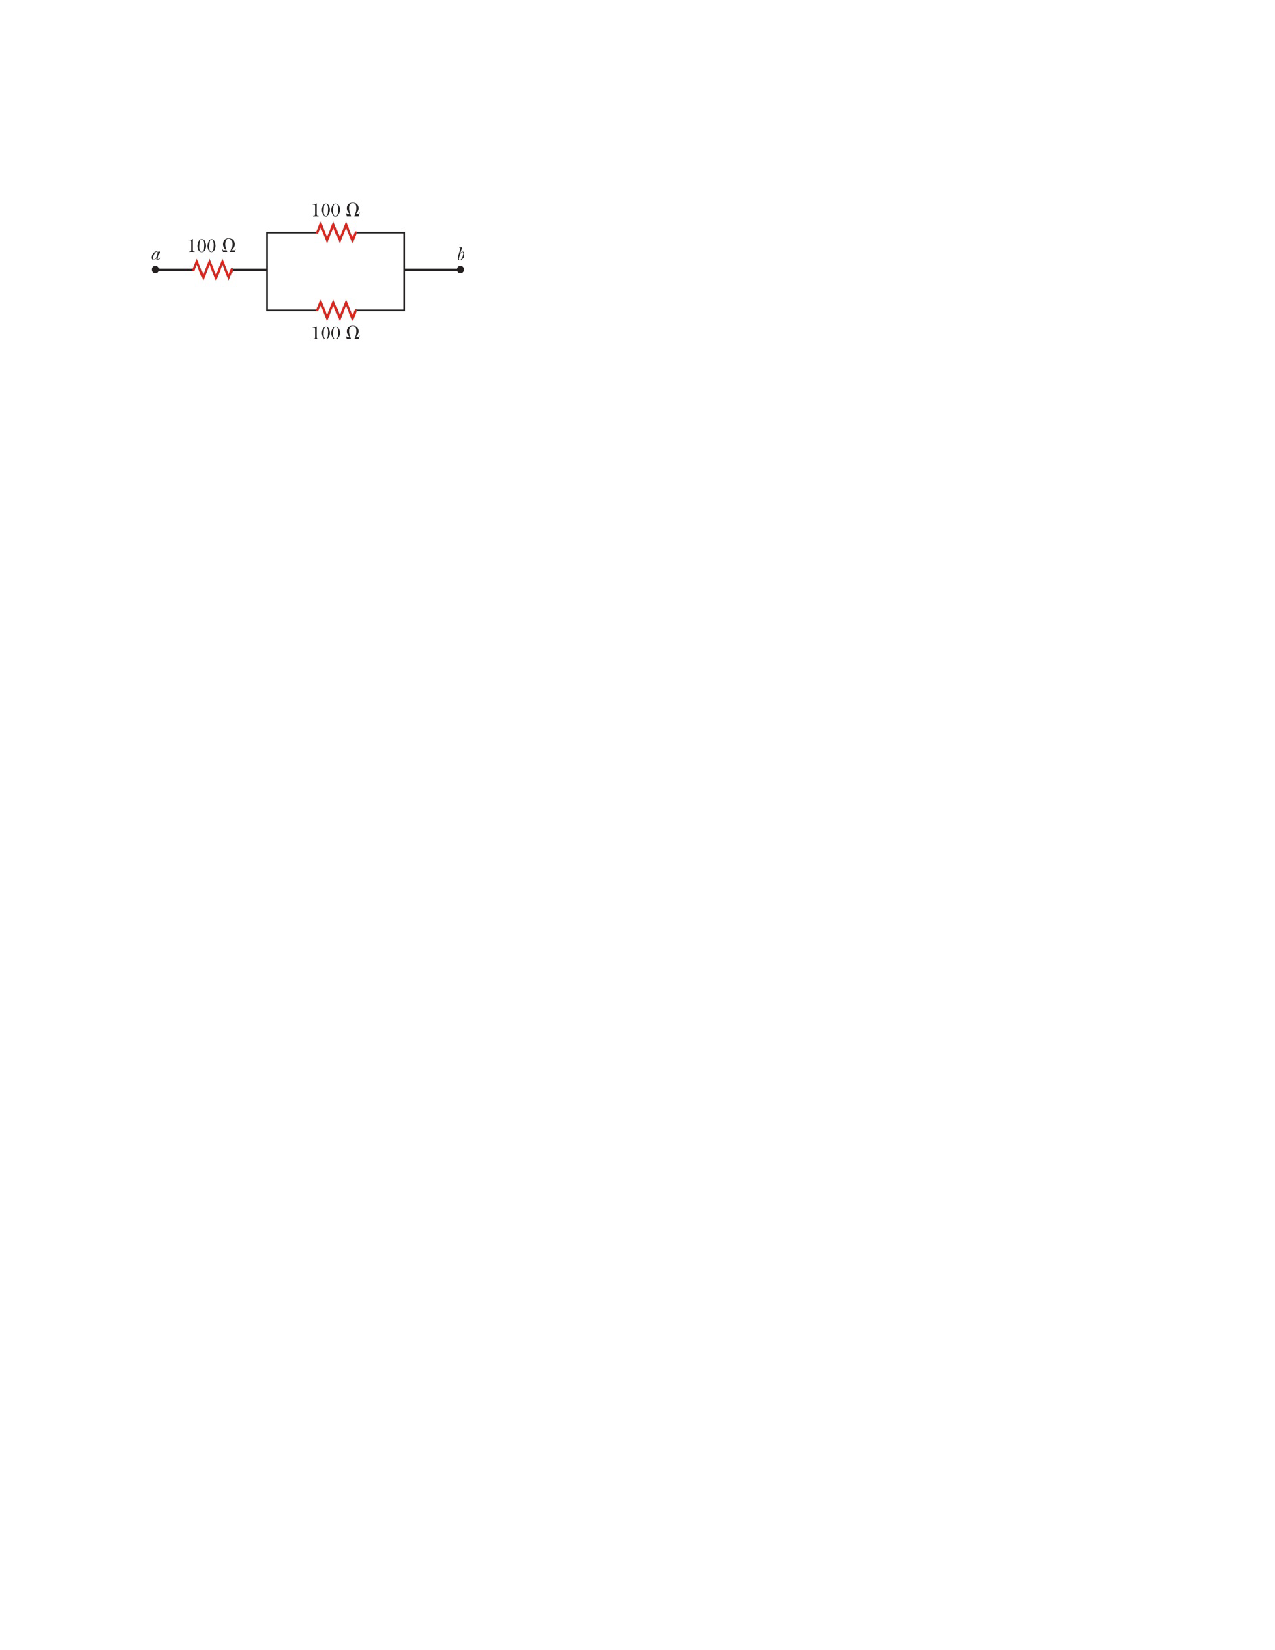
\includegraphics{M_problems/circuits/three_100_ohm_resistors.pdf}
\end{center}
\end{Exercise}
\begin{Answer}
Hint: It's not obvious which resistor is the limiting factor, so try both possibilities: first \textit{assume} that the one resistor on the left is dissipating its maximum power and see where that gets you.  Then \textit{assume} that one of the two resistors in parallel is dissipating its maximum power, and see where that gets you.  (a) 75 V (b) 37.5 W
\end{Answer}


%--------------------------------------------------------------------------------------------------------------
\begin{Exercise}
Suppose your hair dryer is rated at 1250 watts, and your clothes iron is rated at 900 watts.  
(a)~How much current does each appliance draw when plugged into a standard 120-volt US wall socket?  
(b)~Suppose you plug both of them into two electrical outlets that are connected to the same circuit within your house.  The circuit is protected by a 15-amp circuit breaker.  Will the circuit breaker be tripped?  
(c)~Could you replace the 15-amp circuit breaker with a 20-amp circuit breaker to solve your problems?  
\end{Exercise}
\begin{Answer}
I mean, you \textit{could}, but it would violate the electrical code, and you would be trading in one problem for a much worse problem. 
The whole point of having a circuit breaker is to prevent too much current from flowing in the wires within your walls. 
The 15-amp breaker means that the wiring was designed to safely handle no more than 15 amps.  
Allowing a greater current would risk burning your house down.
\end{Answer}


%--------------------------------------------------------------------------------------------------------------
\figuretoright{0.50}{M_problems/circuits/complex_circuit.pdf}{
\begin{Exercise}
In the circuit shown to the right, find the following: 
(a) The current through the $10\ohm$ resistor. 
(b) The power dissipated in the $8\ohm$ resistor. 
(c) The power supplied by the battery. 
(d) The potential difference between points A and B shown in the figure.  
(e) If the wire breaks at point B, does the current through resistor $R_1$ increase, decrease or stay the same?
\end{Exercise}
\begin{Answer}
(a) 0.25 amps, (b) 0.5 watts (c) 2.5 watts (d)~1.75 volts (e)~decreases
\end{Answer}
}

%--------------------------------------------------------------------------------------------------------------
\begin{Exercise}
In class, we charged up a large, $130,000~\mu$F capacitor to a potential of 100~volts.  We then discharged it quickly by touching two wires together---so quickly, in fact, that it made a giant spark and welded the two wires together.  
(a)~Suppose that the actual discharge took place over a time of about one tenth of a second.  What was the average current in the wire during the time of the discharge? 
(b)~Suppose the wires had a cross sectional area of one square millimeter and were made of copper.  Assuming one free electron per copper atom and a density of $8.5 \times 10^{28}$ atoms per cubic meter, what was the average velocity $v_\text{D}$ of the electrons in the wire during the discharge? 
(c)~Are you surprised that the velocity is so small?
\end{Exercise}
\begin{Answer}
(a) 130 Amps.  (b) About 1 cm/sec. (c) Yes, you are surprised.
\end{Answer}


%--------------------------------------------------------------------------------------------------------------
\begin{Exercise}
A $22~\mu$F capacitor is initially charged to a potential of 10~volts, is discharged through a $27\kohm$ resistor. 
(a)~What is the time constant $\tau$ of the RC circuit?  
(b)~How long does it take for the voltage across the capacitor to decrease from 10~volts to 2~volts?  
(c)~At that time, what are the charges on the positive and negative plates of the capacitor?  
(d)~When the capacitor is fully discharged, a switch is flipped that connects the capacitor through the same $27\kohm$ resistor to a 10~V power supply.  
How long does it take for the capacitor's voltage to reach 9~volts?  
(e)~How long would it take for the capacitor's voltage to reach 9~volts if it had started at 2~volts? \end{Exercise}
\begin{Answer}
(a) 0.594 seconds (b) 0.95 seconds (c) $\pm44~\mu$C (d) 1.37 seconds (e) 1.24 seconds
\end{Answer}


%--------------------------------------------------------------------------------------------------------------
\figuretoright{0.50}{M_problems/circuits/cylindrical_capacitor.pdf}{
\begin{Exercise}
\label{cylindrical_capacitor_problem}
A \textit{cylindrical capacitor} consists of two concentric cylinders.  
The inner cylinder is a solid conductor of radius $a$.  
The outer cylinder is a thin cylindrical shell (meaning it's hollow), and has inner radius $b$.  
The cylinders both have a length $L$ that is \textit{much} longer than either of their radii, so you can safely treat them as infinitely long.  
(a)~Suppose the inner cylinder has charge $+Q$, and the outer cylinder has charge $-Q$.  
Find the electric field in between the cylinders, at some radius $r$ where $a<r<b$.  
(b)~Based on your answer in part (a), find the potential difference $\Delta V$ between the two cylinders.  
(c)~What is the capacitance of this device? 
\end{Exercise}
\begin{Answer}
(b) $\displaystyle \Delta V=\frac{Q \ln{(b/a)}}{2\pi \epsilon_0 L}$   
(c) $\displaystyle C=\frac{2\pi \epsilon_0 L}{\ln{(b/a)}}$
\end{Answer}
}

%--------------------------------------------------------------------------------------------------------------
\begin{Exercise}
\label{problem_designing_a_capacitor}
You want to design a parallel-plate capacitor with a capacitance of 0.25~nF that can withstand a potential difference of 600~volts, but you want to make it as small and cheap as possible.  
For a dielectric material in between the plates, you will use Mylar, which has a dielectric constant $\kappa=3.1$ and a dielectric strength $E_\text{max}=7\times10^6$~V/m. 
(a) What is the smallest possible separation $d$ between the plates that will still prevent charge from jumping between the plates at the maximum voltage (also called \textit{dielectric breakdown})?  
(b) What is the minimum area $A$ of the plates required?  
(c) What would be the smallest volume of Mylar required to make the capacitor?  
\end{Exercise}
\begin{Answer}
(a) $85~\mu$m (c) 67 cubic millimeters
\end{Answer}


%--------------------------------------------------------------------------------------------------------------
\begin{Exercise}
A cylindrical capacitor, as in problem~\ref{cylindrical_capacitor_problem}, has radii $a=1.1$~mm, $b=3.1$~mm, and a length of $L=4$~m.  
It is filled with Teflon (PTFE) as a dielectric material, which has $\kappa=2.1$ and a dielectric strength of $E_\text{max}=1.9\times 10^7$~V/m.  
In this problem, you will find the maximum voltage we can place across the capacitor without bad stuff happening.  
\begin{enumerate}[label=(\alph*), nosep, topsep=-2ex, after={\vspace{2ex}}]
\item In problem~\ref{cylindrical_capacitor_problem}, you found that the capacitance of a cylindrical capacitor is given by $C=2\pi\epsilon_0 L/\ln(b/a)$.   How does this expression change if the capacitor is filled with a dielectric with constant $\kappa$?
\item If a charge is placed on the capacitor (say, $+Q$ on the inside, $-Q$ on the outside) where is the electric field strongest: at $r=a$, at $r=b$, or is it uniform everywhere?  
\item Use Gauss' law to write an expression for $E$ at the surface of the inner conductor, $r=a$, in terms of $Q, a, L, \kappa$ and $\epsilon_0$.  
\item Numerically, what is the largest value of $Q$ you can place on the inner conductor without exceeding the dielectric strength of the Teflon?  
\item What is the maximum voltage $V_\text{max}$ you can put across this capacitor without exceeding $E_\text{max}$ of the Teflon?  Hint: you can use your result from part~(a).  
\item In problem~\ref{problem_designing_a_capacitor}, we used the relationship that $V_\text{max}=E_\text{max} d$, where $d$ was the separation between the two electrodes (the two plates).  Here, the separation between the electrodes is 2~mm.  Numerically, is $V_\text{max}=E_\text{max} (b-a)$ true here?  Why or why not?
\end{enumerate}
\end{Exercise}
\begin{Answer}
(a) $\displaystyle C=\frac{2\pi\epsilon_0 \kappa L}{\ln(b/a)}$
(b)~strongest at $r=a$.  
(c) $\displaystyle E=\frac{Q}{2\pi\epsilon_0 \kappa aL}  $
(d)~$9.76~\mu$C  
(e)~21.65~kV 
(f)~No; that expression would give 38~kV, almost twice the $V_\text{max}$ you found in part e.  The expression we used for the parallel plates is invalid here because the electric field is not uniform in between the cylinders.
\end{Answer}


%--------------------------------------------------------------------------------------------------------------
\begin{Exercise}
A 22 picofarad capacitor consists of two parallel plates separated by an air gap of 2~mm.  
To increase its capacitance, the center is filled with a molten wax which, when solidified, has a dielectric constant of 3.5.  
However, in doing so, the gap between the plates is inadvertently expanded from 2~mm to 2.5~mm.  (a)~What is the new capacitance of the wax-filled capacitor, and (b)~what is the area of the plates?
\end{Exercise}




\vspace{0.7in}

\textbf{Answers to Selected {\thesubsection} Problems:}
\label{circuit_prob_answers}
%\shipoutExercise
\shipoutAnswer

\cleardoublepage
